%% %%%%%%%%%%%%%%%%%%%%%%%%%%%%%%%%%%%%%%%%% %%
%% Elementos Pré Textuais
%% ----------------------
%% 
%% Segundo o manual do IFPI, eles devem ser os seguintes (nessa ordem):
%%  1. Capa (obrigatório)
%%  2. Folha de rosto (obrigatório)
%%  3. Errata (opcional)
%%  4. Folha de aprovação (obrigatório)
%%  5. Dedicatória (opcional)
%%  6. Agradecimentos (opcional)
%%  7. Epígrafe (opcional)
%%  8. Resumo (obrigatório)
%%  9. Abstract/Resumo em outra língua (obrigatório)
%% 10. Lista de Ilustrações (opcional)
%% 11. Lista de Tabelas (opcional)
%% 12. Lista de Abreviaturas e Siglas (opcional)
%% 13. Lista de Símbolos (opcional)
%% 14. Sumário (obrigatório)
%% %%%%%%%%%%%%%%%%%%%%%%%%%%%%%%%%%%%%%%%%% %%

%% 01: Capa
\imprimircapa



%% 02: Folha de Rosto
%% OBS: O asterisco indica que haverá ficha bibliográfica (só funciona para impressão frente-e-verso)
\imprimirfolhaderosto*



%% Ficha Catalográfica (acho que é melhor adicionar via \includepdf depois)
%% Ficha Catalográfica
%%
%% Este template cria um quadro semelhante a ficha catalográfica oficial.
%% É melhor usar \includepdf depois que a ficha oficial estiver em mãos.

%% Caso tenha o arquivo PDF da ficha
%% A ficha catalográfica do IFPI pode ser gerada através neste link: https://sistemas.ifpi.edu.br/fichacatalografica/
%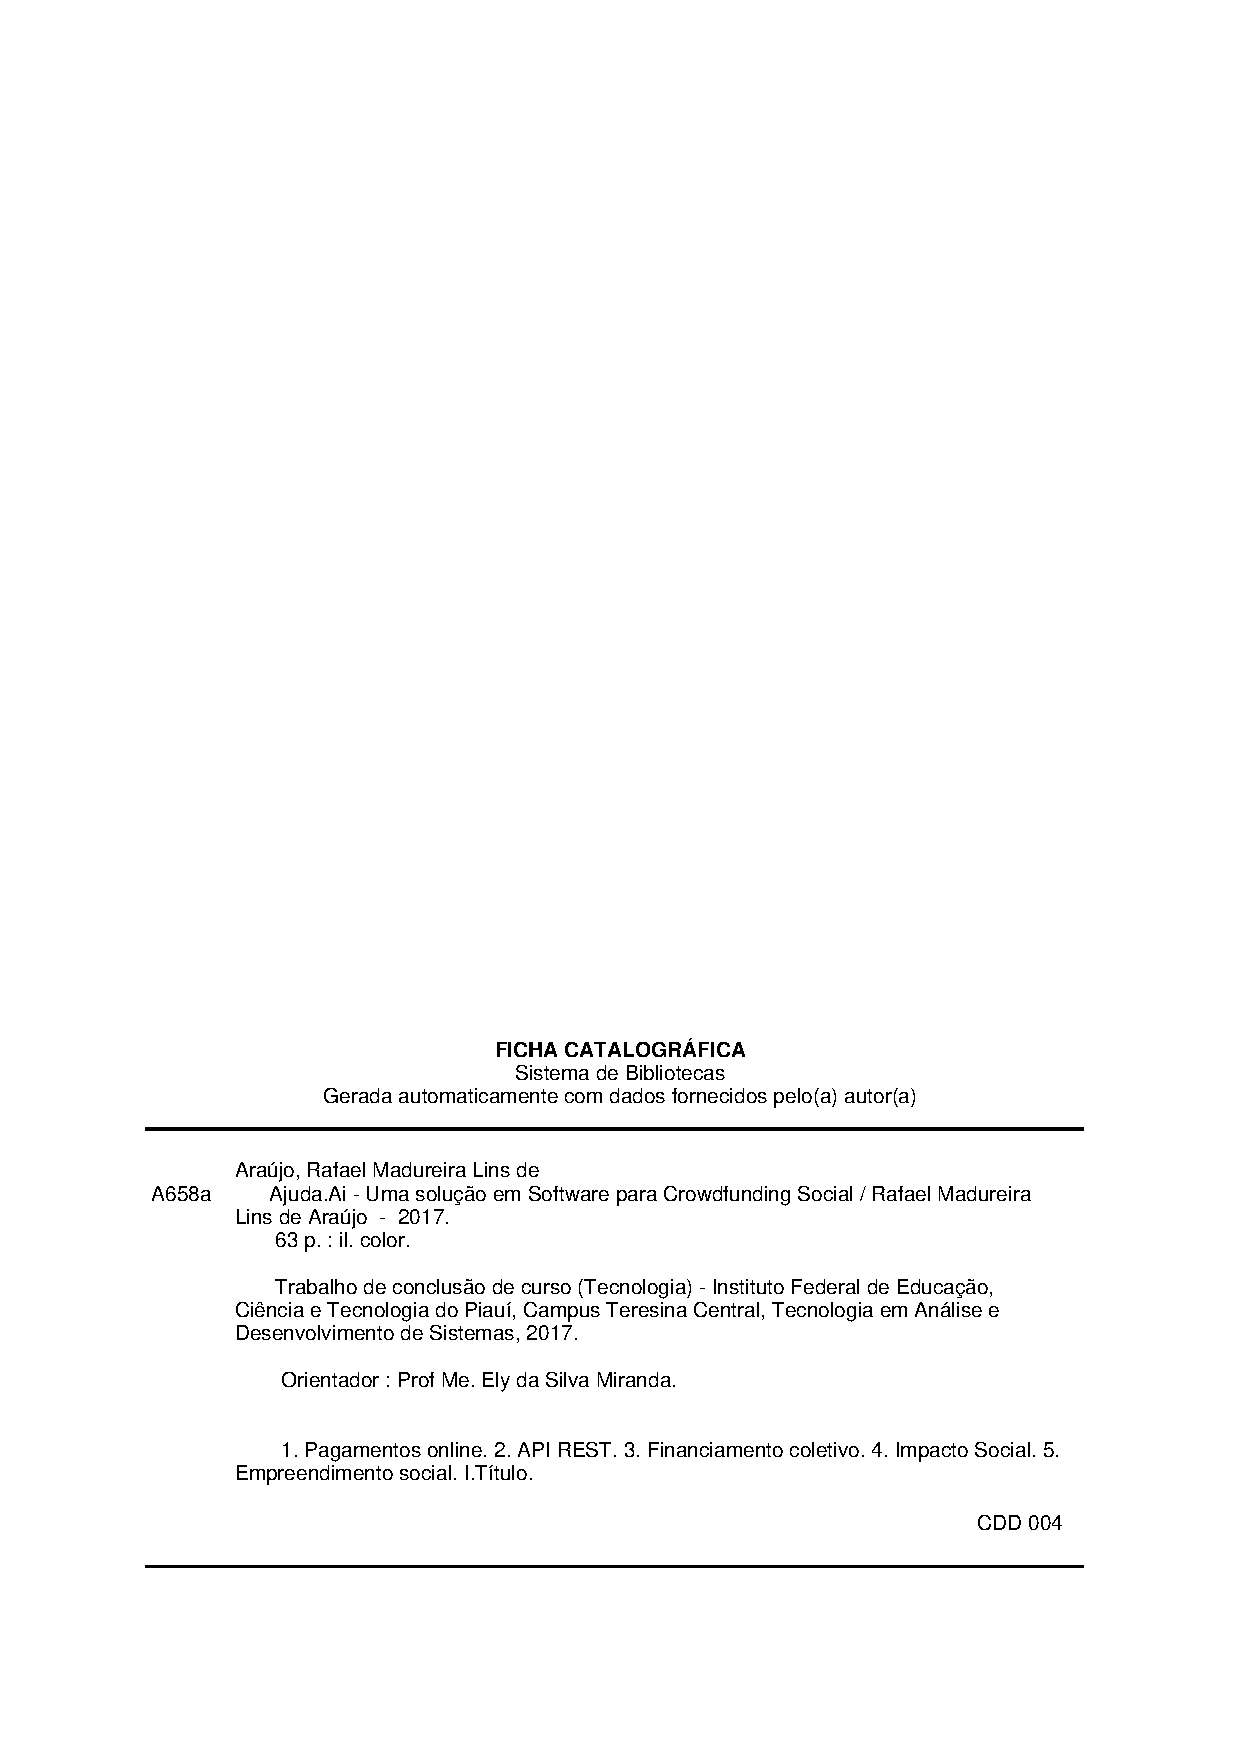
\includepdf{pre-textual/ficha-catalografica.pdf}

%% Caso queira fazer a ficha "tradicional" (este serve apenas como um modelo)
%\begin{fichacatalografica}
%	\sffamily
%	\vspace*{\fill}					% Posição vertical
%	\begin{center}					% Minipage Centralizado
%	\fbox{\begin{minipage}[c][8cm]{13.5cm}		% Largura
%	\small
%	\imprimirautor
%	
%	\hspace{0.5cm} \imprimirtitulo  / \imprimirautor. --
%	\imprimirlocal, \imprimirdata-
%	
%	\hspace{0.5cm} \thelastpage p. : il. (algumas color.) ; 30 cm.\\
%	
%	\hspace{0.5cm} \imprimirorientadorRotulo~\imprimirorientador\\
%	
%	\hspace{0.5cm}
%	\parbox[t]{\textwidth}{\imprimirtipotrabalho~--~\imprimirinstituicao,
%	\imprimirdata.}\\
%	
%	\hspace{0.5cm}
%		1. Palavra-chave1.
%		2. Palavra-chave2.
%		2. Palavra-chave3.
%		I. Orientador.
%		II. Universidade xxx.
%		III. Faculdade de xxx.
%		IV. Título 			
%	\end{minipage}}
%	\end{center}
%\end{fichacatalografica}


%% 03: Errata
%% Errata
%\begin{errata}
%Elemento opcional da norma ABNT NBR14724 de 2011. Exemplo:
%
%\vspace{\onelineskip}
%
%FERRIGNO, C. R. A. \textbf{Tratamento de neoplasias ósseas apendiculares com reimplantação de enxerto ósseo autólogo autoclavado %associado ao plasma rico em plaquetas}: estudo crítico na cirurgia de preservação de membro em cães. 2011. 128 f. Tese (Livre-Docência) %- Faculdade de Medicina Veterinária e Zootecnia, Universidade de São Paulo, São Paulo, 2011.

%% Tabela de exemplo com os erros
%\begin{table}[htb]
%\center
%\footnotesize
%\begin{tabular}{|p{1.4cm}|p{1cm}|p{3cm}|p{3cm}|}
%  \hline
%   \textbf{Folha} & \textbf{Linha}  & \textbf{Onde se lê}  & \textbf{Leia-se}  \\
%    \hline
%    1 & 10 & auto-conclavo & autoconclavo\\
%   \hline
%\end{tabular}
%\end{table}
%
%\end{errata}



%% 04: Folha de Aprovação
\imprimirfolhadeaprovacao
%% Use esta se forem 4 membros na banca:
%\imprimirfolhadeaprovacaoduascolunas



%% 05: Dedicatória
%%% Dedicatória do seu trabalho
%\begin{dedicatoria}
%	%% Empura o texto a seguir para a parte de baixo da página
%	\vspace*{\fill}
%    
%    %% Alinhado a Direita
%    \center
%    \begin{flushright}
%    	Dedico este trabalho à minha família.
%    \end{flushright}
%    
%    %% Descomente a linha seguir para deixar o texto centralizado verticalmente na página
%    %% Lembre de comentar o "\begin{}" e "\end{}" acima para centralizar o texto da dedicatória.
%	%\vspace*{\fill}
%%\end{dedicatoria}



%% 06: Agradecimentos
%% Agradecimentos
\begin{agradecimentos}
Agradeço aos meus pais, que me incentivaram e me apoiaram durante todo meu processo educacional e no meu dia-a-dia.  Aos meus familiares, que mesmo não estando próximos, sempre perguntavam como estavam meus estudos, minha vida.

Também agradeço todos os outros professores que passaram pela minha vida educacional, aos companheiros de trabalho, que sempre que precisava de alguma ajuda, estavam lá para me ajudar resolver o problema juntos. Não menos importante, agradeço aos meus amigos, os quais fizeram grande diferença na minha vida e que jamais serão esquecidos.

A todos que , independente da forma , fizeram parte da minha formação, o meu muito obrigado.

\end{agradecimentos}



%% 07: Epígrafe
%% Epígrafe
%% Uma frase que lhe inspira ou a qual lhe inspirou a fazer este trabalho
\begin{epigrafe}
\vspace*{\fill}
\begin{flushright}
\emph{"Não devemos nos questionar porque algumas coisas nos acontecem e sim o que podemos fazer com o tempo que nos é dado" 
\\ (Senhor dos Anéis – A Sociedade do Anel)}
\end{flushright}
\end{epigrafe}



%% 08: Resumo
%% Resumo
\begin{resumo}
As redes sociais tem como propósito o compartilhamento de conhecimentos e informações. Com a grande popularização da internet as redes sociais se virtualizaram, atendendo as necessidades de comunicação e os relacionamentos da vida real usando o ambiente virtual. Em paralelo a evolução da internet e das redes sociais, outra area que obteve grande crescimento foi o vegetarianismo e veganismo. Grande parte dos adeptos deste regime alimentar iniciam essa prática devido as questões relacionadas a saúde, economia, ambiente, ética e religião. Em busca de uma alimentação adequada, muitos seguidores optam em começar a fazer suas próprias refeições ao invés buscarem em restaurantes. O presente trabalho apresenta o desenvolvimento de um aplicativo mobile implementado na plataforma híbrida Ionic, que produz código executável para os ambientes operacionais IOS 7+ e Android 4.2+, além de integrada ao Facebook. O aplicativo irá funcionar como uma rede social, onde os usuários poderão publicar receitas, disponibilizá-las para todos que estiverem usando o aplicativo. Poderão curtir, favoritar e comentar na receita publicada como também seguir quem publicou a receita, criando assim, um vínculo social dentro do aplicativo.

\vspace{\onelineskip}
\noindent\\
\textbf{Palavras-chaves}: Redes sociais, vegetarianismo, veganismo, aplicativo mobile, Ionic, IOS, Android, Facebook.
\end{resumo}

%% 09: Abstract/Resumo em língua estrangeira
%% Abstract (configurado para língua inglesa)
\begin{resumo}[Abstract]			% Título do Resumo (Abstract = Resumo em inglês)
\begin{otherlanguage*}{english}		% Língua do texto
  The purpose of social networks is to share knowledge and information. With the great popularization of the Internet, social networks have become virtualized, meeting the needs of communication and real-life relationships using the virtual environment. In parallel to the evolution of the internet and social networks, another area that has grown enormously was vegetarianism and veganism. Many of the adherents of this diet begin this practice due to issues related to health, economy, environment, ethics and religion. In pursuit of adequate food, many followers choose to start making their own meals rather than going to restaurants. The present work presents the development of a mobile application implemented in the Ionic hybrid platform, which produces executable code for the IOS 7+ and Android 4.2+ operating environments, as well as integrated with Facebook. The application will act as a social network, where users can post recipes, make them available to everyone who is using the app. They can enjoy, favor and comment on the published recipe as well as follow who posted the recipe, thus creating a social bond within the application.
  
\vspace{\onelineskip}
\noindent\\
\textbf{Keywords}: Social networks, vegetarianism, veganism, mobile application, Ionic, IOS, Android, Facebook.
\end{otherlanguage*}
\end{resumo}

%% Exemplo de resumo em francês
%\begin{resumo}[Résumé]
% \begin{otherlanguage*}{french}
%    Il s'agit d'un résumé en français.
% 
%   \textbf{Mots-clés}: latex. abntex. publication de textes.
% \end{otherlanguage*}
%\end{resumo}

%% Exemplo de resumo em Espanhol
%\begin{resumo}[Resumen]
% \begin{otherlanguage*}{spanish}
%   Este es el resumen en español.
%  
%   \textbf{Palabras clave}: latex. abntex. publicación de textos.
% \end{otherlanguage*}
%\end{resumo}
% ---



%% 10: Lista de Ilustrações
%% Lista de Ilustrações
\pdfbookmark[0]{\listfigurename}{lof}
\listoffigures*
\cleardoublepage



%% 11: Lista de Tabelas
%% Lista de Tabelas
\pdfbookmark[0]{\listtablename}{lot}
\listoftables*
\cleardoublepage





%% 12: Lista de Abreviaturas e Siglas
%%% Lista de Siglas
\begin{siglas}
  \item[CDN] CONTENT DELIVERY NETWORK
  \item[CSS] CASCADING STYLE SHEETS
  \item[HTTP] HYPERTEXT TRANSFER PROTOCOL 
  \item[HTML] HYPERTEXT MARKUP LANGUAGE 
  \item[IDE] INTEGRATED DEVELOPMENT ENVIRONMENT 
  \item[IP] INTERNET PROTOCOL 
  \item[PEP] PYTHON ENHANCEMENT PROPOSAL 
  \item[P2P] PEER TO PEER
  \item[RSS] REALLY SIMPLE SYNDICATION
  \item[WSGI] WEB SERVER GATEWAY INTERFACE
  \item[WWW] WORLD WIDE WEB 
  \item[ARPA] ADVANCED RESEARCH PROJECT AGENCY
  \item[ORM] OBJECT-RELATIONAL MAPPING
\end{siglas}



%% 13: Lista de Símbolos
%%% Lista de Símbolos
%% (esta é apenas uma lista de exemplo)
%\begin{simbolos}
%  \item[$ \Gamma $] Letra grega Gama
%  \item[$ \Lambda $] Lambda
%  \item[$ \zeta $] Letra grega minúscula zeta
%  \item[$ \in $] Pertence
%\end{simbolos}



%% 14: Sumário (o asterisco retira o próprio sumário do sumário)
\pdfbookmark[0]{\contentsname}{toc}
\tableofcontents*
\cleardoublepage